\subsection{Architectural Description}
The software architecture is comprised of several subsystems, which have different responsibilities in the system.

\begin{figure}
	\centering
	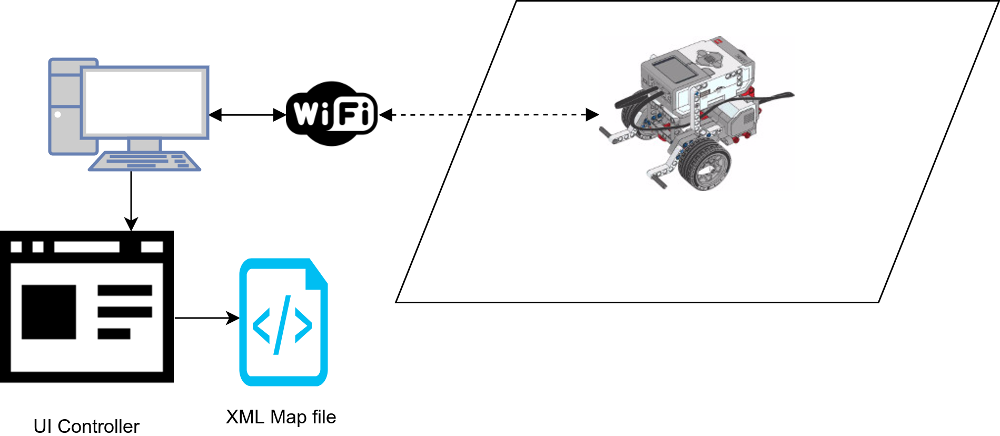
\includegraphics[width=0.9\textwidth]{Robot_system.png}
	\caption{\label{fig:robotSystem}This needs to be updated though}
\end{figure}   

\subsection{Component Decomposition Description}
The system has been broken down into clearly defined components, which can be tested individually. Each of these components perform a function in the entire system.

\begin{tabular}{|c|l|}
	\hline
	\bf{Location} & \bf{Description} \\
	\hline
	\hline
	Ev3 Robot & Embedded control software \\
	\hline
	PC & UI display \\
	\hline
	PC & Robot Control Services \\
	\hline
	PC & Robot State Logic \\
	\hline
\end{tabular}

\subsection{Detailed Components Design Description}

\subsubsection{C00 Lejos Library}\label{compLejos}
\begin{itemize}
	\item Purpose:
	\item Function: To interface to the robot.
	\item Subordinates: \nameref{compMove}, \nameref{compSense}
	\item Dependencies:
	\item Interfaces:
	\begin{itemize}
		\item
	\end{itemize}
	\item Data:
\end{itemize}

\subsubsection{C01 Movement Service} \label{compMove}
\begin{itemize}
	\item Purpose: To provide a simple abstraction to move the robot.
	\item Function: 
	\item Subordinates: \nameref{compState}
	\item Dependencies: \nameref{compLejos}
	\item Interfaces:
	\begin{itemize}
		\item
	\end{itemize}
	\item Data:
\end{itemize}

\subsubsection{C02 Sensors Service} \label{compSense}
\begin{itemize}
	\item Purpose: To provide a simple abstraction to receive sensor readings from the robot.
	\item Function: 
	\item Subordinates: \nameref{compState}
	\item Dependencies: \nameref{compLejos}, \nameref{compShared}
	\item Interfaces:
	\begin{itemize}
		\item
	\end{itemize}
	\item Data:
\end{itemize}

\subsubsection{C03 Robot State Machine} \label{compState}
\begin{itemize}
	\item Purpose: A logic to defined the logic of the system.
	\item Function:
	\item Subordinates: \nameref{compUI}
	\item Dependencies: \nameref{compShared}, \nameref{compMove}, \nameref{compSense}
	\item Interfaces:
	\begin{itemize}
		\item
	\end{itemize}
	\item Data:
\end{itemize}

\subsubsection{C04 Shared Core} \label{compShared}
\begin{itemize}
	\item Purpose: This is a component to share interfaces between other components, like models and service instances.
	\item Function:
	\item Subordinates: \nameref{compState}, \nameref{compUI}, \nameref{compSense}, \nameref{compUIUpdater}, \nameref{compMove}
	\item Dependencies: Null
	\item Interfaces:
	\begin{itemize}
		\item
	\end{itemize}
	\item Data:
\end{itemize}

\subsubsection{C05 User Interface} \label{compUI}
\begin{itemize}
	\item Purpose: To provide an interactive display of the system to the user.
	\item Function: 
	\item Subordinates: \nameref{compUIUpdater}
	\item Dependencies: \nameref{compState}, \nameref{compShared}
	\item Interfaces:
	\begin{itemize}
		\item
	\end{itemize}
	\item Data:
\end{itemize}

\subsubsection{C06 UI Updater} \label{compUIUpdater}
\begin{itemize}
	\item Purpose: To constantly update parts of the GUI in real time.
	\item Function: 
	\item Subordinates:
	\item Dependencies: \nameref{compUI}, \nameref{compState}, \nameref{compShared}
	\item Interfaces:
	\begin{itemize}
		\item
	\end{itemize}
	\item Data:
\end{itemize}

\subsection{Architectural Alternatives}
\subsection{Design Rationale}